\documentclass[12pt,a4paper,onecolumn]{exam}

\usepackage{amsmath}
\usepackage{amsthm}
\usepackage{amssymb}
\usepackage{graphicx}
\usepackage{float}
\usepackage{geometry}
\usepackage{tikz}
\usepackage[skins]{tcolorbox}
\usepackage{listings}
\usepackage{xcolor}
\usepackage{hyperref}
\usepackage{multirow}
\usepackage{adjustbox}
\usepackage{booktabs}
\usepackage[font=small]{caption}
\usepackage{subcaption}

% --- Code Listing Colors ---
\definecolor{codegreen}{rgb}{0,0.6,0}
\definecolor{codegray}{rgb}{0.5,0.5,0.5}
\definecolor{codepurple}{rgb}{0.58,0,0.82}
\definecolor{backcolour}{rgb}{0.95,0.95,0.92}

% --- Code Listing Style ---
\lstdefinestyle{mystyle}{
    backgroundcolor=\color{backcolour},
    commentstyle=\color{codegreen},
    keywordstyle=\color{magenta},
    numberstyle=\tiny\color{codegray},
    stringstyle=\color{codepurple},
    basicstyle=\ttfamily\footnotesize,
    breaklines=true,
    captionpos=b,
    keepspaces=true,
    numbers=left,
    numbersep=2pt,
    showspaces=false,
    showstringspaces=false,
    showtabs=false,
    tabsize=1
}

\newcommand{\questionheader}[1]{%
  \begin{tcolorbox}[
    enhanced,
    colback=black,
    coltext=white,
    boxrule=0pt,
    fontupper=\Large\bfseries,
    arc=4mm
  ]
  #1
  \end{tcolorbox}%
}

\lstset{style=mystyle, language=Python}
\raggedbottom

\begin{document}

\begingroup
    \centering
    \LARGE E1 244 Detection and Estimation Theory\\
    \LARGE Assignment 7\\[0.5em]
    \large Dwaipayan Haldar\par
    \large \today\\[0.5em]
\endgroup
\noindent\rule{\textwidth}{0.5pt}
\printanswers
\renewcommand{\solutiontitle}{\noindent\textbf{Ans:}\enspace}

%----------------------------------------------------------------------
\questionheader{Problem 1}
%----------------------------------------------------------------------

\begin{solution}

\[
\mathbb{E}[C(H_0,\theta)\mid y=y]
=\int_{\theta\in\Theta} C(H_0,\theta)f(\theta\mid y)\,d\theta
\]
\[
=\int_{\theta\in X_0} C(H_0,\theta)f(\theta\mid y)\,d\theta
+\int_{\theta\in X_1} C(H_0,\theta)f(\theta\mid y)\,d\theta
\]
\[
=\int_{0.5}^{1} \frac{1}{\theta}\,f(\theta\in X_1\mid y)\,d\theta.
\]

\[
f(\theta\in X_1\mid y)
=\frac{f(y\mid \theta\in X_1)f(\theta\in X_1)}{f(y)}
\]
\[
=\frac{f(y\mid \theta\in X_1,H_1)\,f(\theta\in X_1\mid H_1)\,f(H_1)}{f(y)}.
\]

So,
\[
\mathbb{E}[C(H_0,\theta)\mid y=y]
=\int_{0.5}^{1}\frac{1}{\theta}\cdot
\theta e^{-\theta y}\mathbf{1}_{\{y\ge 0\}}\cdot
2\mathbf{1}_{\{0.5\le \theta\le 1\}}\cdot\frac{1}{2}\cdot\frac{1}{f(y)}\,d\theta
\]
\[
=\frac{\mathbf{1}_{\{y\ge 0\}}}{f(y)}\int_{0.5}^{1}e^{-\theta y}\,d\theta
=\frac{\mathbf{1}_{\{y\ge 0\}}}{f(y)}\left[\frac{e^{-\theta y}}{-y}\right]_{0.5}^{1}
\]
\[
=\frac{\mathbf{1}_{\{y\ge 0\}}}{y f(y)}\left(e^{-y/2}-e^{-y}\right).
\]

Also,
\[
\mathbb{E}[C(H_1,\theta)\mid y=y]
=\int_{\theta\in X_0} f(\theta\mid y)\,d\theta
=\frac{f(y\mid \theta)}{f(y)}
=\frac{1}{2}\frac{e^{-y/2}}{f(y)}\mathbf{1}_{\{y\ge 0\}}.
\]

So, the Bayes rule:
\[
\frac{e^{-y/2}(1-e^{-y/2})\mathbf{1}_{\{y\ge0\}}}{y f(y)}
\underset{H_0}{\overset{H_1}{\gtrless}}
\frac{1}{2}\frac{e^{-y/2}}{f(y)}\mathbf{1}_{\{y\ge0\}}
\]
\[
\Rightarrow\quad
\frac{1-e^{-y/2}}{y/2}
\underset{H_0}{\overset{H_1}{\gtrless}}1,
\quad y\ge0.
\]

\[
\frac{1-e^{-y/2}}{y/2}<1,\ \forall y>0,
\qquad
\text{at }y=0\ \text{it is a tie}.
\]

So,
\[
\forall y>0,\ \text{choose }\delta(y)=H_0;
\qquad
\text{at }y=0,\ \text{choose }\delta(y)=H_1\ (\text{any choice}).
\]

\[
\bar J(y)=
\begin{cases}
\mathbb{E}[C(H_0,\theta)\mid y=y], & \delta(y)=H_0,\\
\mathbb{E}[C(H_1,\theta)\mid y=y], & \delta(y)=H_1.
\end{cases}
\]

\[
J(\delta)=\int_{R_0}\bar J(y)f(y)\,dy+\int_{R_1}\bar J(y)f(y)\,dy,
\]
where
\[
R_0=\{y:\delta(y)=H_0\},\quad R_1=\{y:\delta(y)=H_1\}.
\]

Thus,
\[
J(\delta)=\int_{R_0}\mathbb{E}[C(H_0,\theta)\mid y=y]f(y)\,dy
+\int_{R_1}\mathbb{E}[C(H_1,\theta)\mid y=y]f(y)\,dy
\]
\[
=\int_{0}^{\infty}\frac{e^{-y/2}-e^{-y}}{y f(y)}f(y)\,dy
=\int_{0}^{\infty}\left(\frac{e^{-y/2}}{y}-\frac{e^{-y}}{y}\right)dy.
\]

\end{solution}

%----------------------------------------------------------------------
\questionheader{Problem 2}
%----------------------------------------------------------------------

\begin{solution}

\textbf{(a)}\quad $H_0:\theta=0$, $H_1:\theta=\theta_1$.

\[
f(y\mid H_0)=\prod_{i=1}^{N}f(y_i\mid H_0)
=\frac{1}{(2\pi)^{N/2}}\exp\left(-\frac{1}{2}\sum_{i=1}^{N}y_i^2\right).
\]

\[
f(y\mid H_1)=\prod_{i=1}^{N}f(y_i\mid H_1)
=\frac{\exp\left(-\frac{1}{2}\sum_{i=1}^{N}\frac{y_i^2}{1+\theta_1^2 s_i^2}\right)}{(2\pi)^{N/2}\prod_{i=1}^{N}(1+\theta_1^2 s_i^2)^{1/2}}.
\]

\[
L(y)=\frac{f(y\mid H_1)}{f(y\mid H_0)}
=\frac{\exp\left(-\frac{1}{2}\left[\sum_{i=1}^{N}\frac{y_i^2}{1+\theta_1^2 s_i^2}-\sum_{i=1}^{N}y_i^2\right]\right)}{\prod_{i=1}^{N}(1+\theta_1^2 s_i^2)^{1/2}}.
\]

\[
L(y)\underset{H_0}{\overset{H_1}{\gtrless}}\gamma
\]
\[
\Rightarrow\quad
-\frac{1}{2}\sum_{i=1}^{N}\left[\frac{y_i^2}{1+\theta_1^2 s_i^2}-y_i^2\right]
-\frac{1}{2}\sum_{i=1}^{N}\ln(1+\theta_1^2 s_i^2)
\underset{H_0}{\overset{H_1}{\gtrless}}\ln\gamma
\]
\[
\Rightarrow\quad
\sum_{i=1}^{N}y_i^2\left[1-\frac{1}{1+\theta_1^2 s_i^2}\right]
\underset{H_0}{\overset{H_1}{\gtrless}}
2\ln\gamma+\sum_{i=1}^{N}\ln(1+\theta_1^2 s_i^2).
\]

Define
\[
T(y)=\sum_{i=1}^{N}\frac{\theta_1^2 s_i^2}{1+\theta_1^2 s_i^2}y_i^2,
\qquad
\eta=2\ln\gamma+\sum_{i=1}^{N}\ln(1+\theta_1^2 s_i^2).
\]
So NP test is $T(y)\underset{H_0}{\overset{H_1}{\gtrless}}\eta$.

\[
T(y)=\sum_{i=1}^{N}a_i y_i^2,
\quad a_i=\frac{\theta_1^2 s_i^2}{1+\theta_1^2 s_i^2},
\]
which is generalized chi-square.

Let
\[
z_i=\frac{y_i}{\sqrt{1+\theta_1^2 s_i^2}},\quad z_i\sim\mathcal{N}(0,1),
\]
then
\[
T(y)=\sum_{i=1}^{N}\theta_1^2 s_i^2 z_i^2=\sum_{i=1}^{N}b_i z_i^2,
\quad b_i=\theta_1^2 s_i^2.
\]

\[
P_F=\int_{\eta}^{\infty} f_{T\mid H_0}(t)\,dt,
\qquad
P_D(\theta)=\int_{\eta}^{\infty} f_{T\mid H_1}(t)\,dt.
\]

So NP test: $\max\ P_D$ s.t. $P_F\le\alpha$.

\textbf{(b)}\quad $H_0:\theta=0$ versus $H_1:\theta>0$.

We have scalar parameter $\theta$.
For any $\theta_0\in\bar\Theta_0=\{0\}$, $\theta_1\in\bar\Theta_1=[0,\infty)$,
\[
L(y;\theta_0,\theta_1)=\frac{f(y\mid\theta_1)}{f(y\mid\theta_0)}
=\frac{\exp\left(\frac{1}{2}\sum_{i=1}^{N}y_i^2\frac{\theta_1^2 s_i^2}{1+\theta_1^2 s_i^2}\right)}{\prod_{i=1}^{N}(1+\theta_1^2 s_i^2)^{1/2}}
\quad (\text{using }\theta_1\text{ constant}).
\]

The UMP would exist when $s_1=s_2=\cdots=s_N=s>0$.
Then $T(y)=\sum y_i^2$ and $L(y;\theta_0,\theta_1)$ is a non-decreasing function in $T(y)$.

Then UMP exists of the form
\[
\sum_{i=1}^{N}y_i^2\underset{H_0}{\overset{H_1}{\gtrless}}\gamma,
\]
where $\gamma$ is selected s.t. $P_F=\alpha$:
\[
P_F=\int_{\gamma}^{\infty} f(T\mid H_0)\,dT
=1-\text{cdf of chi-square}(\gamma).
\]
So,
\[
\gamma=F_N^{-1}(1-P_F)\quad [F_N\ \text{is cdf of chi-square}],
\]
and
\[
T(y)\underset{H_0}{\overset{H_1}{\gtrless}}F_N^{-1}(1-\alpha).
\]

\textbf{(c)}\quad GLRT assuming $s_1=s_2=\cdots=s_N=s$.

\[
\hat\theta_0=0,
\qquad
\hat\theta_1=\arg\sup_{\theta\in\Theta_1}f(y\mid\theta)
=\arg\sup_{\theta\in\Theta_1}
\frac{\exp\left(-\frac{1}{2(1+\theta^2 s^2)}\sum_{i=1}^{N}y_i^2\right)}{(2\pi)^{N/2}(1+\theta^2 s^2)^{N/2}}.
\]

Differentiating and setting to 0, with
\[
p^2=\frac{1}{1+\theta^2 s^2},\qquad T(y)=\sum y_i^2,
\]
we get (as in derivation)
\[
N=T(y)\,p
\Rightarrow p=\frac{N}{T(y)}
\Rightarrow 1+\theta^2 s^2=\frac{T(y)}{N}
\Rightarrow \theta=\frac{1}{s^2}\left(1-\frac{T(y)}{N}\right).
\]

GLRT:
\[
\frac{f(y\mid\hat\theta_1)}{f(y\mid\hat\theta_0)}\underset{H_0}{\overset{H_1}{\gtrless}}\gamma
\]
\[
\frac{\left(\frac{N}{T(y)}\right)^{N/2}\exp\left(-\frac{1}{2}\frac{N}{T(y)}\,T(y)\right)}{\exp\left(-\frac{1}{2}T(y)\right)}
\underset{H_0}{\overset{H_1}{\gtrless}}\gamma
\]
\[
\left(\frac{N}{T(y)}\right)^{N/2}\exp\left(-\frac{1}{2}N\right)\exp\left(\frac{1}{2}T(y)\right)
\underset{H_0}{\overset{H_1}{\gtrless}}\gamma
\]
\[
\frac{e^{-\frac{1}{2}T(y)}}{T(y)^{N/2}}
\underset{H_0}{\overset{H_1}{\gtrless}}
\frac{\gamma}{\exp\left(-\frac{1}{2}N\right)N^{N/2}}\triangleq\eta.
\]

For $T\ge0$, $\dfrac{e^{-T/2}}{T^{N/2}}$ is a decreasing function.
So final test can be written as
\[
T\underset{H_1}{\overset{H_0}{\gtrless}}T^*,
\]
where $T^*$ is such that
\[
e^{-\frac{1}{2}T^*}=\eta\,(T^*)^{N/2}.
\]

\end{solution}

%----------------------------------------------------------------------
\questionheader{Problem 3}
%----------------------------------------------------------------------

\begin{solution}

\textbf{(a)}

\[
y=H\theta+w.
\]
When $\theta\ne0$, $y\mid\theta\sim\mathcal{N}(H\theta,\sigma^2 I)$.
So,
\[
f(y\mid\theta)=L(\theta)=k\exp\left[-\frac{1}{2}(y-H\theta)^T(\sigma^2 I)^{-1}(y-H\theta)\right].
\]

\[
\hat\theta_1(y)=\arg\max_{\theta\ne0}f(y\mid\theta)
=\arg\min_{\theta\ne0}\|y-H\theta\|_2^2
=(H^TH)^{-1}H^Ty.
\]

\textbf{(b)}\quad GLRT
\[
\frac{\sup_{\theta\ne0}f(y\mid\theta)}{f(y\mid0)}\underset{H_0}{\overset{H_1}{\gtrless}}\gamma,
\qquad
f(y\mid0)=k\,e^{-\frac{1}{2\sigma^2}\|y\|_2^2}.
\]

\[
\sup_{\theta\ne0}f(y\mid\theta)=k\,e^{-\frac{1}{2\sigma^2}\|y-H\hat\theta(y)\|_2^2}.
\]

So,
\[
e^{-\frac{1}{2\sigma^2}\|y-H\hat\theta(y)\|_2^2+\frac{1}{2\sigma^2}\|y\|_2^2}
\underset{H_0}{\overset{H_1}{\gtrless}}\gamma
\]
\[
\Rightarrow\quad
\frac{1}{2\sigma^2}\left(y^Ty-y^Ty+2\hat\theta(y)^TH^Ty-\hat\theta(y)^TH^TH\hat\theta(y)\right)
\underset{H_0}{\overset{H_1}{\gtrless}}\ln\gamma.
\]

Since
\[
2\hat\theta_1(y)^TH^Ty=\hat\theta_1(y)^TH^TH\hat\theta_1(y)
\quad [\because\ y-H\hat\theta\ \perp\ \text{col}(H)],
\]
we get
\[
s(y)=\frac{\hat\theta_1^T(y)H^TH\hat\theta_1(y)}{\sigma^2}
\underset{H_0}{\overset{H_1}{\gtrless}}\eta.
\]

\textbf{(c)}

\[
\hat\theta(y)=(H^TH)^{-1}H^Ty.
\]

If $y\sim\mathcal{N}(\mu,\sigma^2 I)$, then for any $A$:
\[
Ay\sim\mathcal{N}(A\mu,\sigma^2 AA^T).
\]

Hence
\[
\hat\theta(y)\sim\mathcal{N}\left((H^TH)^{-1}H^T\mu,\ (H^TH)^{-1}\sigma^2\right).
\]
When $\theta=0$,
\[
\hat\theta(y)\sim\mathcal{N}\left(0,(H^TH)^{-1}\sigma^2\right).
\]

By property given in hint,
\[
\frac{\hat\theta^T(y)(H^TH)\hat\theta(y)}{\sigma^2}
\ \text{is chi-squared with }M\ \text{degrees of freedom.}
\]
So,
\[
s(y)\sim\chi_M^2\ \text{under }H_0.
\]

When $\mu\ne0$, similarly $s(y)$ is non-central chi-squared, with noncentrality
\[
\left((H^TH)^{-1}H^TH\theta\right)^T
\left(\frac{H^TH}{\sigma^2}\right)
\left((H^TH)^{-1}H^TH\theta\right)
=\frac{\theta^TH^TH\theta}{\sigma^2}.
\]

Now, if $R$ is P.D., by Cholesky $R=LL^T$.
Define $z=L^{-1}x$.
Then
\[
z\sim\mathcal{N}(L^{-1}\mu,I).
\]

Also,
\[
x^TR^{-1}x=x^T(L^T)^{-1}L^{-1}x=z^Tz=\sum z_i^2.
\]

If $\mu=0$, then $x^TR^{-1}x$ is a $\chi_M^2$ distribution.
If $\mu\ne0$, then $x^TR^{-1}x$ is a non-central $\chi_M^2$ distribution with
\[
\lambda=\sum \mu_i'^2=\mu'^T\mu',\quad \mu'=L^{-1}\mu.
\]
Then,
\[
\mu'^T(L^{-1})^TL^{-1}\mu=\mu^TR^{-1}\mu
\Rightarrow \lambda=\mu^TR^{-1}\mu.
\]

\end{solution}

%----------------------------------------------------------------------
\questionheader{Problem 4}
%----------------------------------------------------------------------

\begin{solution}

\textbf{(a)}

\underline{Test 1:}
\[
P_F=\Pr(H_1\mid H_0).
\]
If $H_0:\theta=0$, then $X_1,X_2\sim$ i.i.d. Uniform$[0,1]$.
\[
\int \mathbf{1}_{\{0.95\le x\le1\}}\,dx_1=0.05.
\]
So, $P_F$ for Test 1 is $0.05$.

\underline{Test 2:}
\[
\Pr(X_1+X_2\ge c),\quad X_1,X_2\sim\text{Uniform}(0,1).
\]
For $1\le c\le2$, the area is
\[
\frac{1}{2}(2-c)(2-c)=\frac{(2-c)^2}{2}.
\]
By problem,
\[
\frac{(2-c)^2}{2}=\alpha
\Rightarrow (2-c)^2=2\alpha
\Rightarrow 2-c=\pm\sqrt{2\alpha}
\Rightarrow c=2\pm\sqrt{2\alpha}.
\]
Since $c\le2$, we take
\[
c=2-\sqrt{2\alpha}.
\]

\begin{figure}[H]
    \centering
    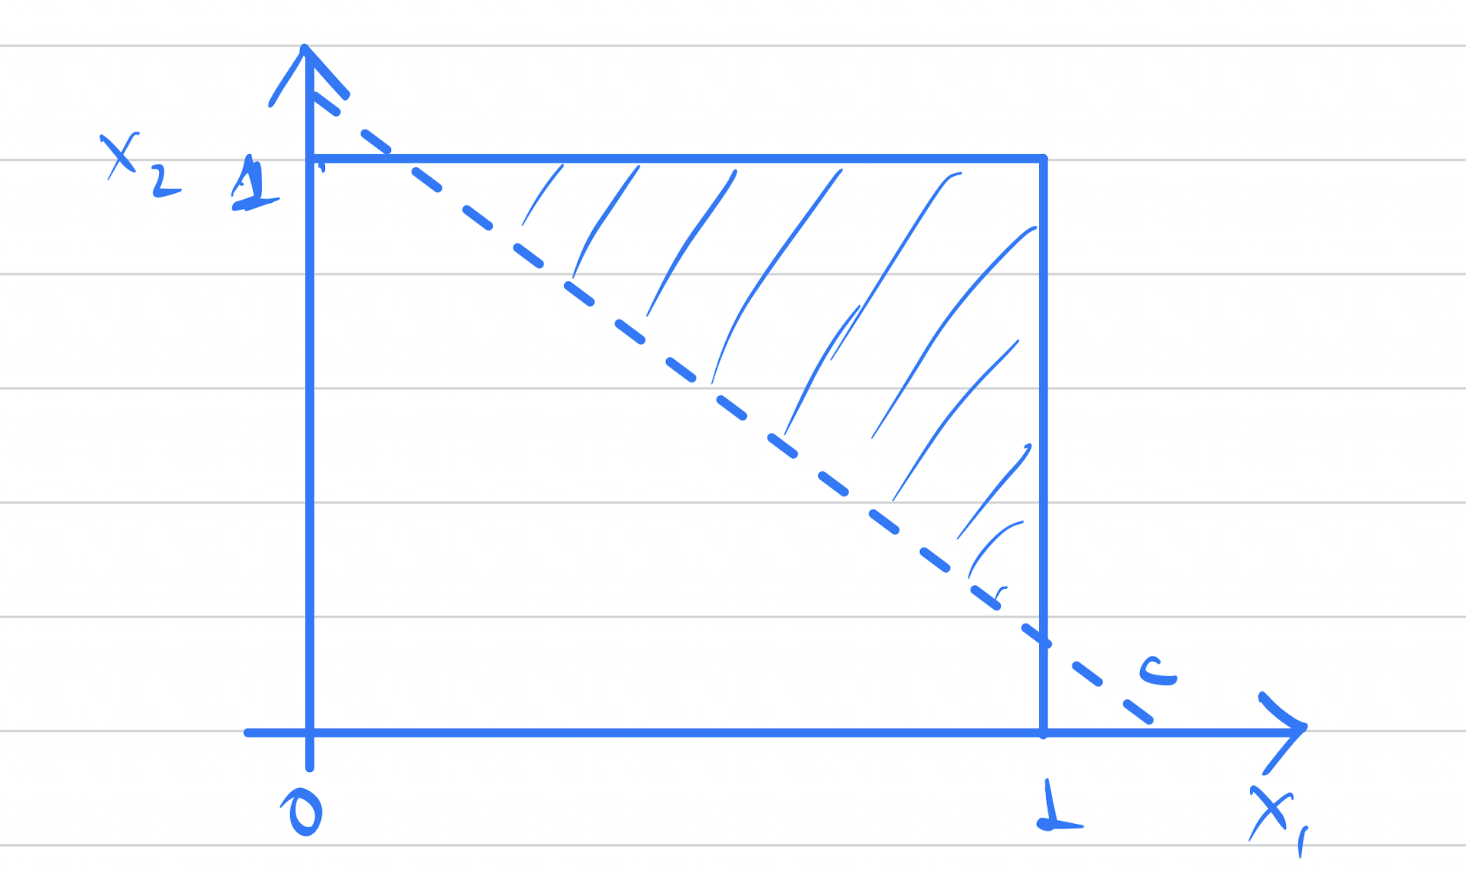
\includegraphics[width=0.52\textwidth]{P04a.png}
    \caption{Area sketch used for computing $\Pr(X_1+X_2\ge c)$ in Problem 4(a).}
    \label{fig:p4a}
\end{figure}

\textbf{(b)}

\underline{Test 1:}
\[
P_D=\Pr(X_1\ge0.95\mid H_1)
=\theta+1-\max\{\theta,0.95\}
=\begin{cases}
1, & \theta\ge0.95,\\
\theta+0.05, & 0\le\theta<0.95.
\end{cases}
\]

\underline{Test 2:}
\[
P_D=\Pr(X_1+X_2\ge c\mid H_1).
\]

If $c\le2\theta$, $P_D(\theta)=1$.
If $c>2\theta+2$, $P_D(\theta)=0$.

For intermediate ranges:
\[
2\theta<c\le2\theta+1\quad\Rightarrow\quad P_D(\theta)=1-\frac{1}{2}(c-2\theta)^2,
\]
\[
2\theta+1<c\le2\theta+2\quad\Rightarrow\quad P_D(\theta)=\frac{1}{2}(2\theta+2-c)^2.
\]

So,
\[
P_D(\theta)=
\begin{cases}
1, & \theta\ge \dfrac{c}{2},\\[6pt]
1-\dfrac{1}{2}(c-2\theta)^2, & \dfrac{c-1}{2}\le\theta<\dfrac{c}{2},\\[8pt]
\dfrac{1}{2}(2\theta+2-c)^2, & \dfrac{c-2}{2}\le\theta<\dfrac{c-1}{2},\\[8pt]
0, & \theta<\dfrac{c-2}{2}.
\end{cases}
\]

\textbf{(c)}

Using
\[
c=2-\sqrt{2\alpha}\approx1.684.
\]

Test 1 is not uniformly most powerful than Test 2.

\begin{figure}[H]
    \centering
    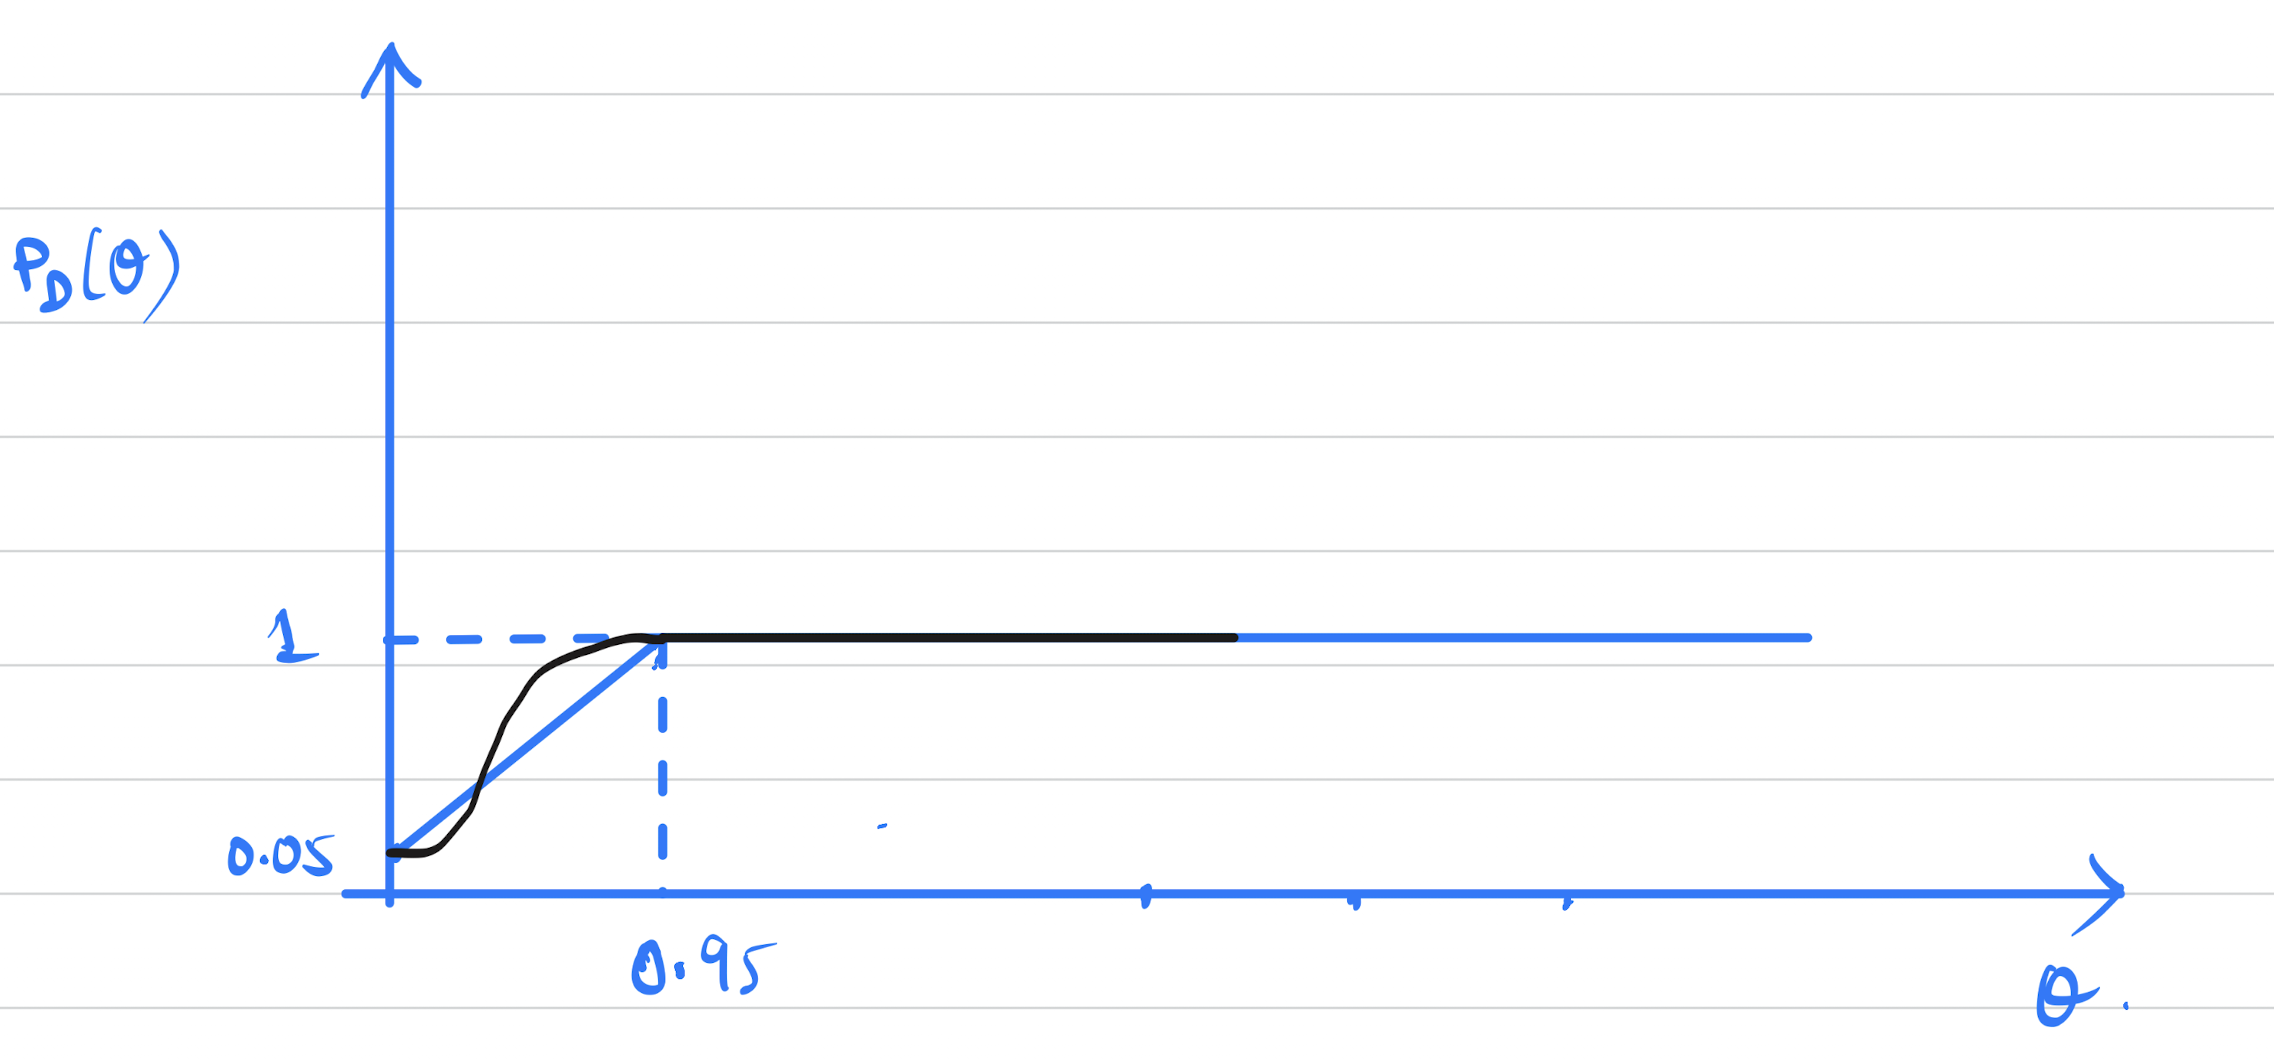
\includegraphics[width=0.60\textwidth]{P04c.png}
    \caption{$P_D(\theta)$ comparison sketch for Test 1 and Test 2 (Problem 4(c)).}
    \label{fig:p4c}
\end{figure}

\end{solution}

\end{document}
